\chapter{Hypothesis Testing}
The final result of this analysis is a measurement of the cross-section for \WR production with subsequent decay for \NR or an upper limit on the cross-section, in the case no signal is observed. By convention, cross-section exclusion limits are set at the 95\% confidence level for this analysis. The calculation of these levels and how the results are interpreted are discussed in this chapter. Limits on the cross-section are calculated use the \CLs technique, which is a modified frequentist approach and the standard technique for limits set by experiments at the \LHC \cite{CLS2002},\cite{smallStatCLs}. Results for the cross-section are presented one dimensionally as a function of \WR mass for both the boosted and resolved \NR case. Two dimensional limits are also shown with resolved and boosted treated separately and combined, where the model $g_{R}=g_{L}$ is assumed.

This analysis considers each bin in the final \WR mass distribution simultaneously. The binning choices for the resolved and boosted analysis are discussed in Chapter \ref{ch:bg_estim}. Inter-bin correlations improve the ability to distinguish signal from background given the \WR mass's peaking behavior. For the heaviest \WR mass that we can set a limit for, however, the last bin influences the limit far more than any other. 

\section{Model Inputs}
To re-summarize the last chapter, and provide all of the raw input information into the statistical calculations, the input distributions are shown here. Each lepton flavor search has three regions, the flavor-sideband, the Drell-Yan control region, and the signal region. Each of these is divided into the two main background components, the other backgrounds, and data.

\section{The \CLs Technique}

\subsection{Overview}
The \CLs technique is a modified frequentist method for setting exclusion limits or establish observations. The frequentist limits used here answer the question, ``How probable is this observation based on a given model''. This is in contrast to Bayesian statistics, which calculate a probability of a model given certain results.

Fundamentally, we can consider two hypotheses. One is that the observed data results from standard model background events. This will be called the null hypothesis, $H_{0}$. The second hypothesis is that the data results from a combination of standard model background events and a new signal, $H_{\mu}$. The variable $\mu$ will be used to represent the amount of signal strength. For this analysis, the signal would be a \WR boson. Now some variable must be selected to allow us to discern between the two hypotheses. This variable is called the test statistic. The total number of events measured in data after some event requirements is an example of a test statistic and is a simplified version of what this analysis uses.

The probability distribution of the test statistic, defined as $q\left(X\right)$, has to be estimated for each of the hypotheses, background only ($H_{0}$) and background + signal ($H_{\mu}$). To estimate the test statistic's distribution for the two hypotheses, toy MC can be used to create many different possible outcomes for $q\left(X\right)$ including all of the uncertainties in the analysis. Once the probability distribution is determined, the probability that the result is caused by background only, $H_{0}$, is
\begin{equation}
    \mathrm{CL}_{b}
    \equiv
    \int\limits_{q\left(X\right)}^{\infty}f\left(0\right)\mathrm{dq}.
\end{equation}

The confidence level for the background only hypothesis, $H_{0}$, is $\mathrm{CL}_{b}$. The probability that the null hypothesis explains a disagreement at least as large as the disagreement between the measured data and the expected background only result is defined as $1-\mathrm{CL}_{b}$. This value is also called the ``p-value''.

The confidence level for the signal + background hypothesis, $\mathrm{CL}_{s+b}$, can be calculated as
\begin{equation}
    \mathrm{CL}_{s+b}
    \equiv
    \int\limits_{q\left(X\right)}^{\infty}f\left(\mu\right)\mathrm{dq}.
\end{equation}
The values of $\mathrm{CL}_{b}$ and $\mathrm{CL}_{s+b}$ can be used to discern between the null hypothesis, $H_{0}$, and the signal + background hypothesis, $H_{\mu}$. The threshold for rejecting the null hypothesis, or the alternative hypothesis, were set by \CMS before any analyses commenced. This removes a potential source of bias in the results. The famous ``$5\sigma$'' threshold is defined as $1-\mathrm{CL}_{b} < 2.87\times10^{-7}$.

Often in searches for new phenomena, no clear evidence for discovery exists in data. Exclusion limits are calculated instead. These limits are calculated based on the confidence interval calculations defined above and are commonly set at the 95th percentile. An exclusion limit is designed to exclude signal by requiring that the probability that the observed data can be described by a background only is less than 5\%. This works out to be $\mathrm{CL}_{s+b}<1-0.95$. Calculating limits in this fashion gives problematic results when backgrounds are much larger than expected signal. The \CLs technique handles this by normalizing the signal + background confidence level with the background only confidence level.
\begin{equation}
    \mathrm{CL}_{S}
    \equiv
    \frac{\mathrm{CL}_{s+b}}{\mathrm{CL}_{b}} < 1-0.95.
\end{equation}

This gives the modified frequentist confidence limit, \CLs. \CLs isn't a true confidence level as it is designed to give values relative to the background confidence level, which are by construction more conservative than $\mathrm{CL}_{s+b}$ alone.

\begin{figure}[!tp]
    \centering
    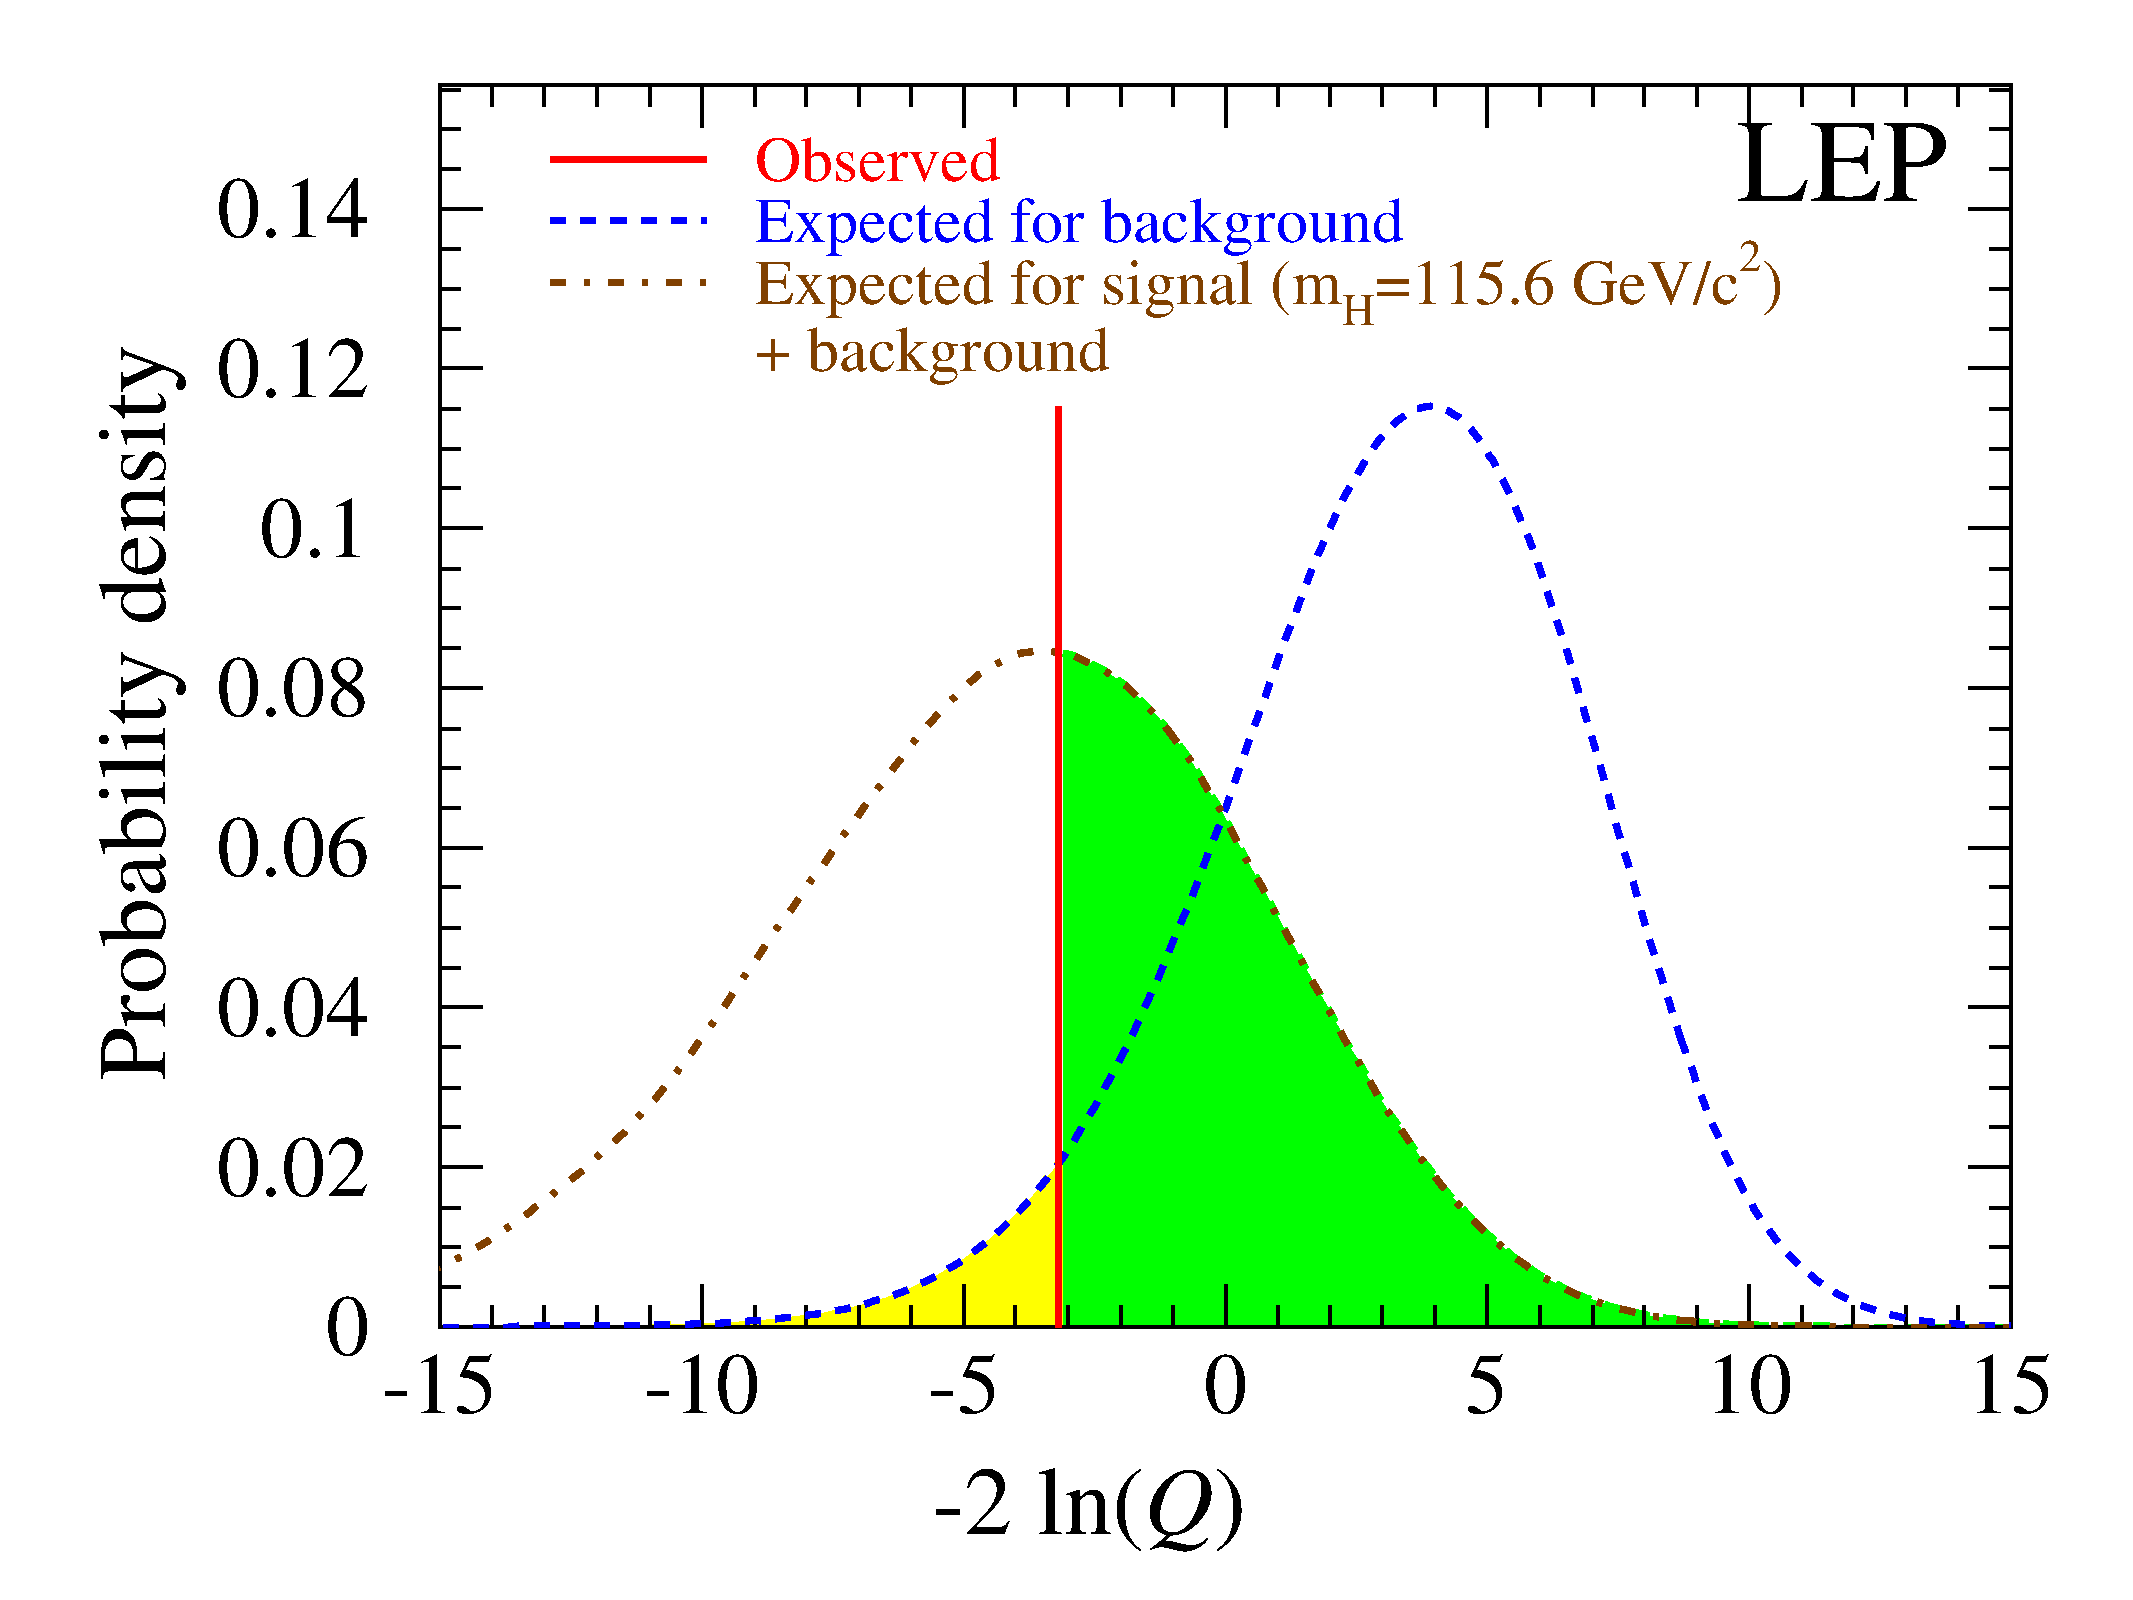
\includegraphics[width=\textwidth]{figures/CLS_2002_plots.pdf}
    \caption[
        %Short caption for the list of figures
       Example likelihood profiles.
    ]{
        % Full caption shown below the image
        An example likelihood profile from a LEP era Higgs search \cite{CLS2002}.
        This plot shows the probability densities for the combined Higgs search at LEP for the background (in blue, on the right) and a
signal + background hypotheses (in gold, on the left) for a previously hypothesized Higgs mass of \ensuremath{\SI{115.6}{GeV/c}} . The yellow region to the left of the observation is $1 − CL_{b}$ and the green region to the right of the observation represents $CL_{s+b}$.
    }
    \label{fig:LEP_CLS_Higgs}
\end{figure}

%\subsection{Higgs Combine} mention, reference, skip
\section{Model Outputs}
After running the statistical fitting, the final signal region distributions are shown HERE. The yields for each contribution to the last bin (the most statistically significant bin) are shown HERE.
\section{Limits}

\subsection{One Dimensional Limits}
To construct one dimensional limits, the relationship of the \NR to the \WR mass is fixed. For the resolved limit, only the \NR with a mass of half of the \WR mass are considered. For the boosted limit, the \NR mass is fixed at \ensuremath{\SI{100}{\GeV}}. This is the lowest mass \NR considered at every \WR mass point, and so it represents the most boosted \WR case for each \WR mass.

\begin{figure}[!tp]
    \centering
    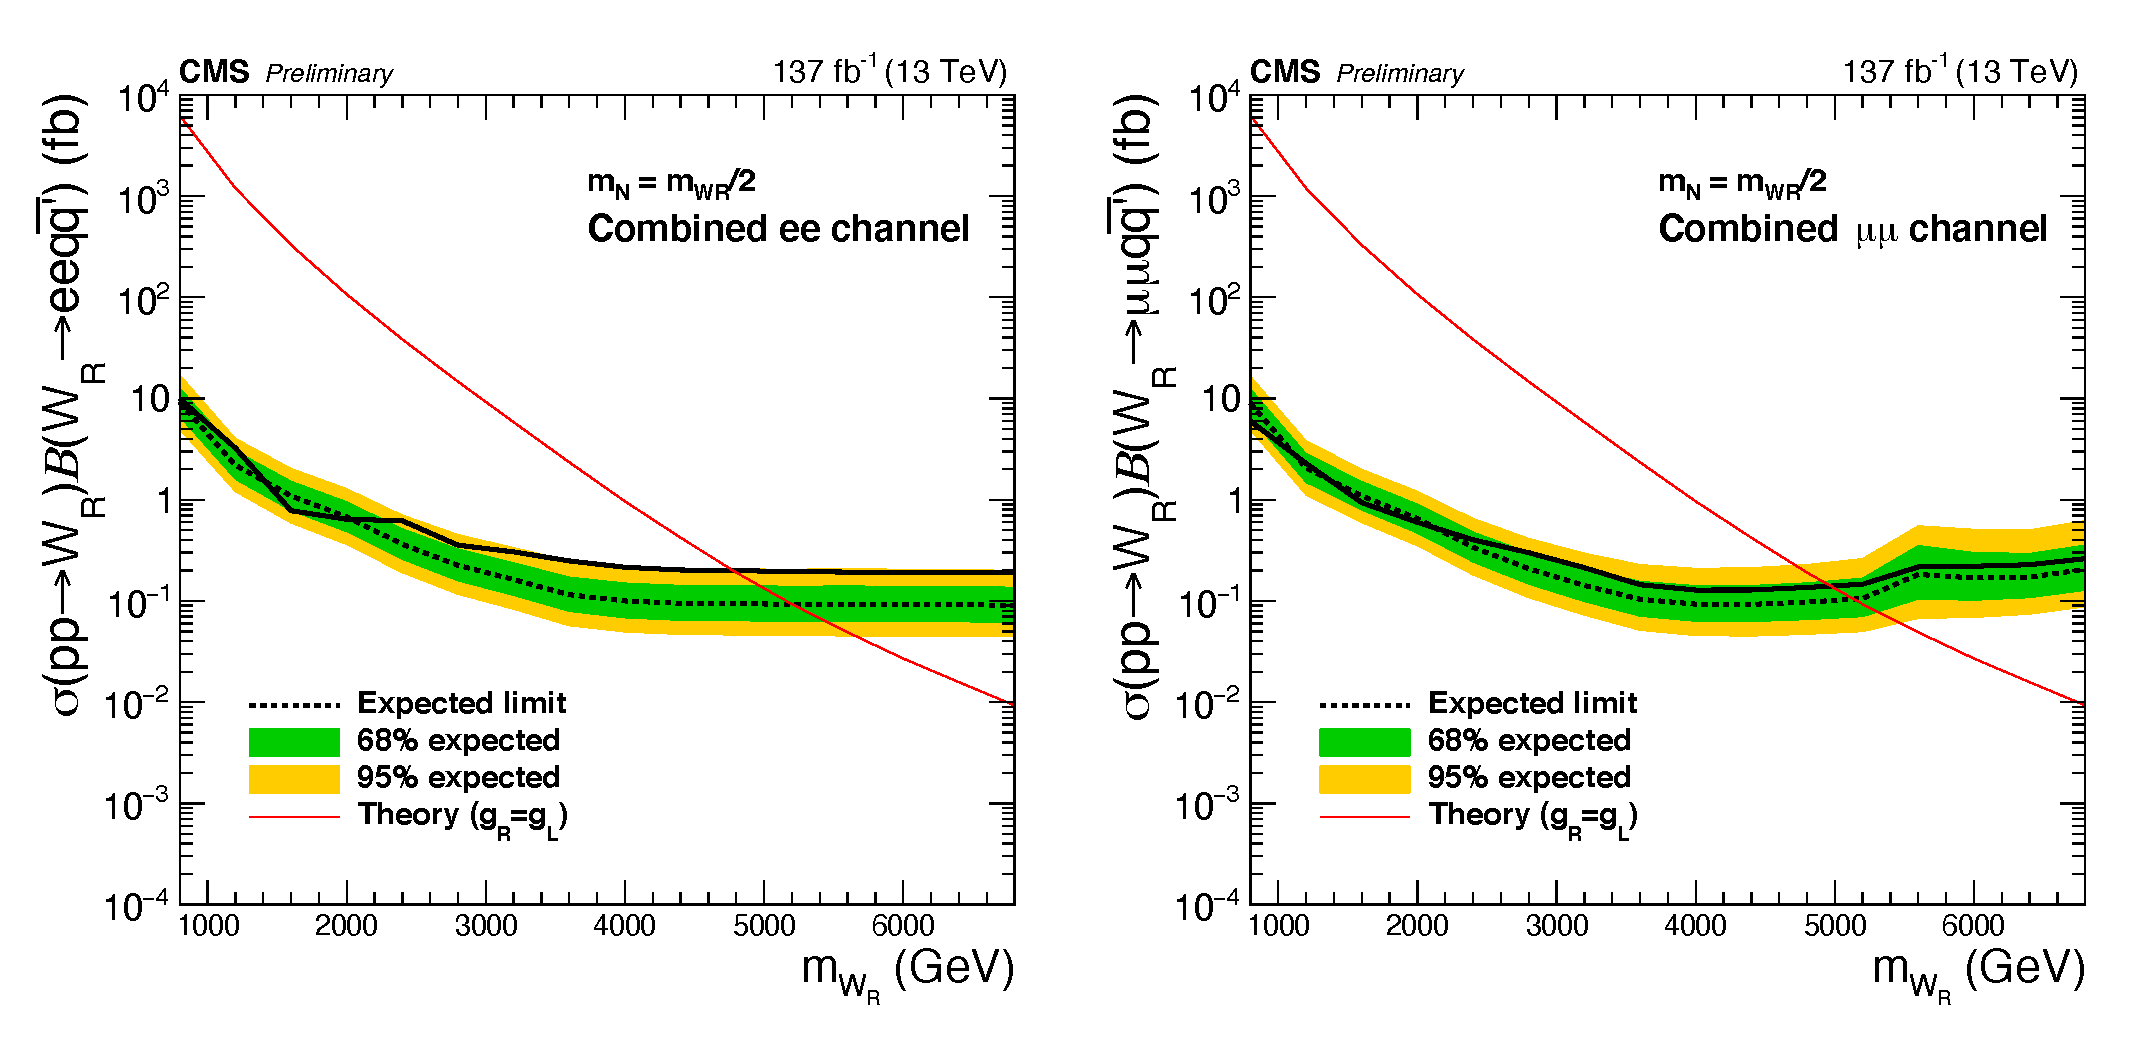
\includegraphics[width=\textwidth]{figures/Results/1D_limit_allYear_unblinded.pdf}
    \caption[
        %Short caption for the list of figures
       1 Dimensional Limits.
    ]{
        % Full caption shown below the image
        The one dimensional limits are shown for both of lepton flavors with the combined data of all three years.  
    }
    \label{fig:1Dlimit}
\end{figure}

\subsection{Two Dimensional Limits}
The two dimensional limits are shown for both searched lepton flavors. Several contours are shown. The resolved and boosted contours are shown separately and combined. It can be seen that the electron channel observed excess results in a worse than expected limit. While the muon channel limit is on the low side of the expected limit, it is important to remember that the observed limit is based on just a few whole events.

%\subsubsection{Resolved}
%\subsubsection{Boosted}
%\subsubsection{Combination}
\begin{figure}[!tbp]
    \centering
    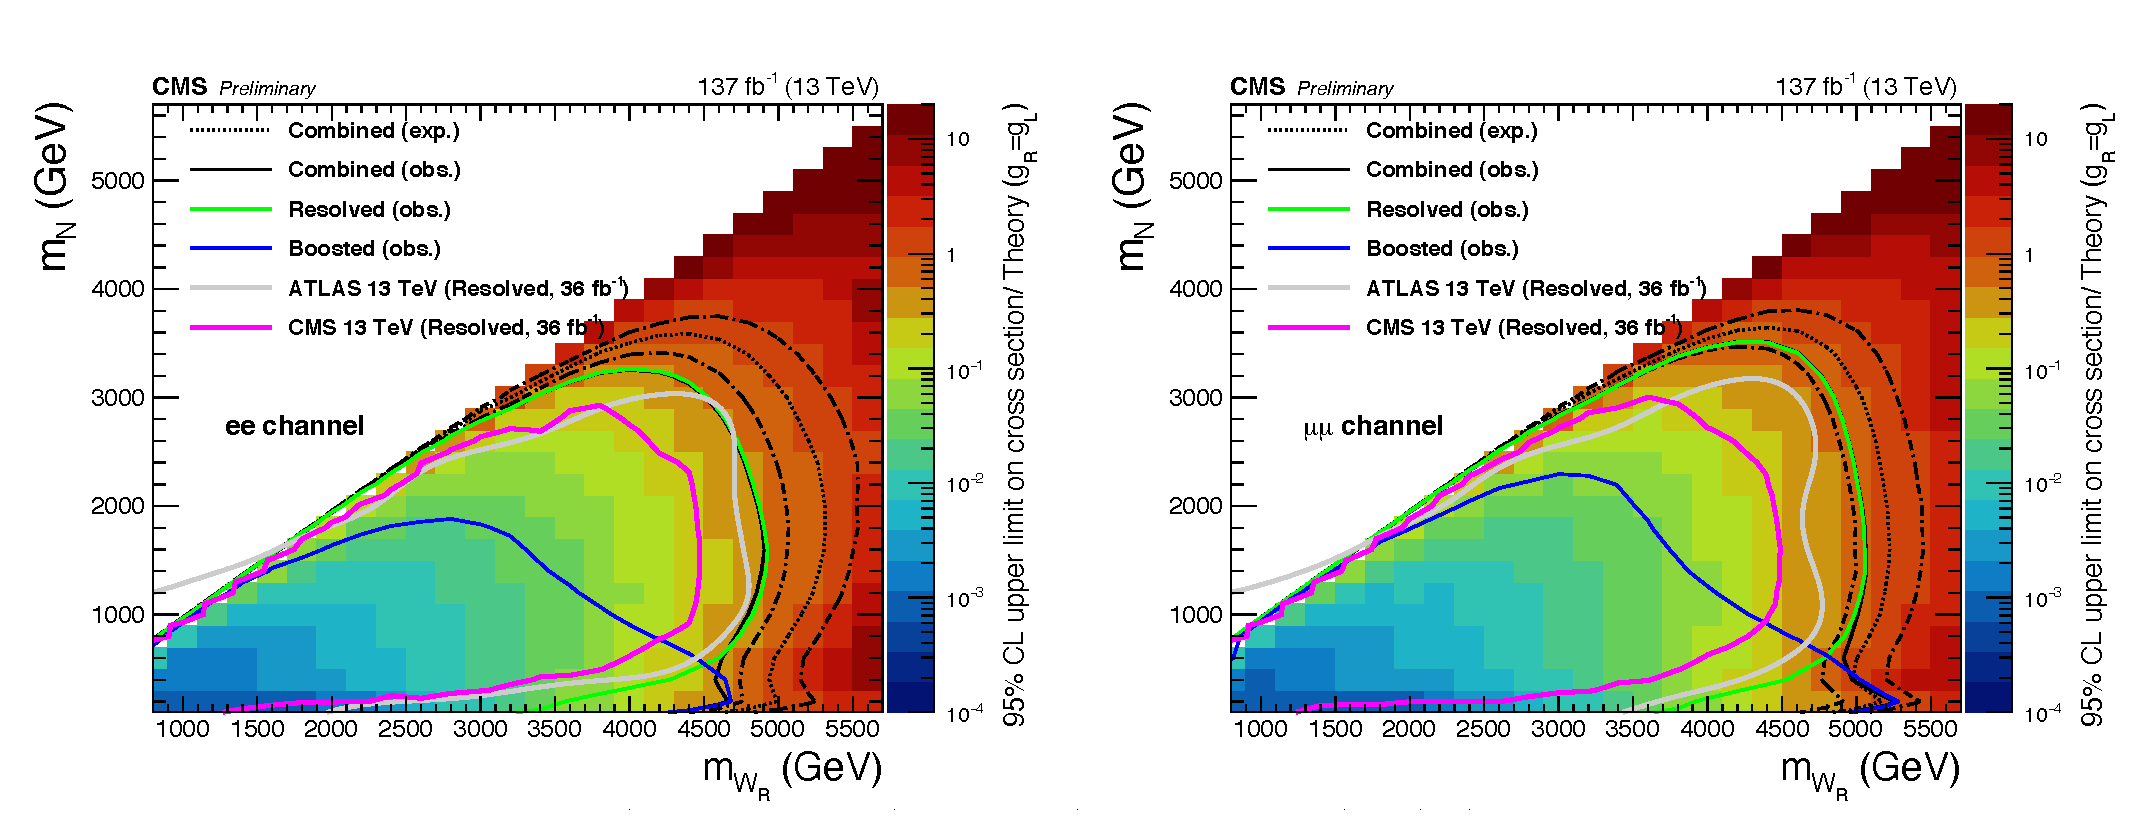
\includegraphics[width=\textwidth]{figures/Results/2D_limit_allyear_unblinded.pdf}
    \caption[
        %Short caption for the list of figures
       2 Dimensional Limits.
    ]{
        % Full caption shown below the image
        The two dimensional limits are shown for both of lepton flavors with the combined data of all three years.  
    }
    \label{fig:1Dlimit}
\end{figure}

\subsection{A Discussion of the Excess}
The electron-flavor analysis shows a roughly two sigma excess in the resolved channel. The expected background distribution for the resolved electron channel for all three years is shown with the data overlayed. A total of thirteen events were observed in the last bin, exceeding the expectation by $\sim 5$ events.

\begin{figure}[!tp]
    \centering
    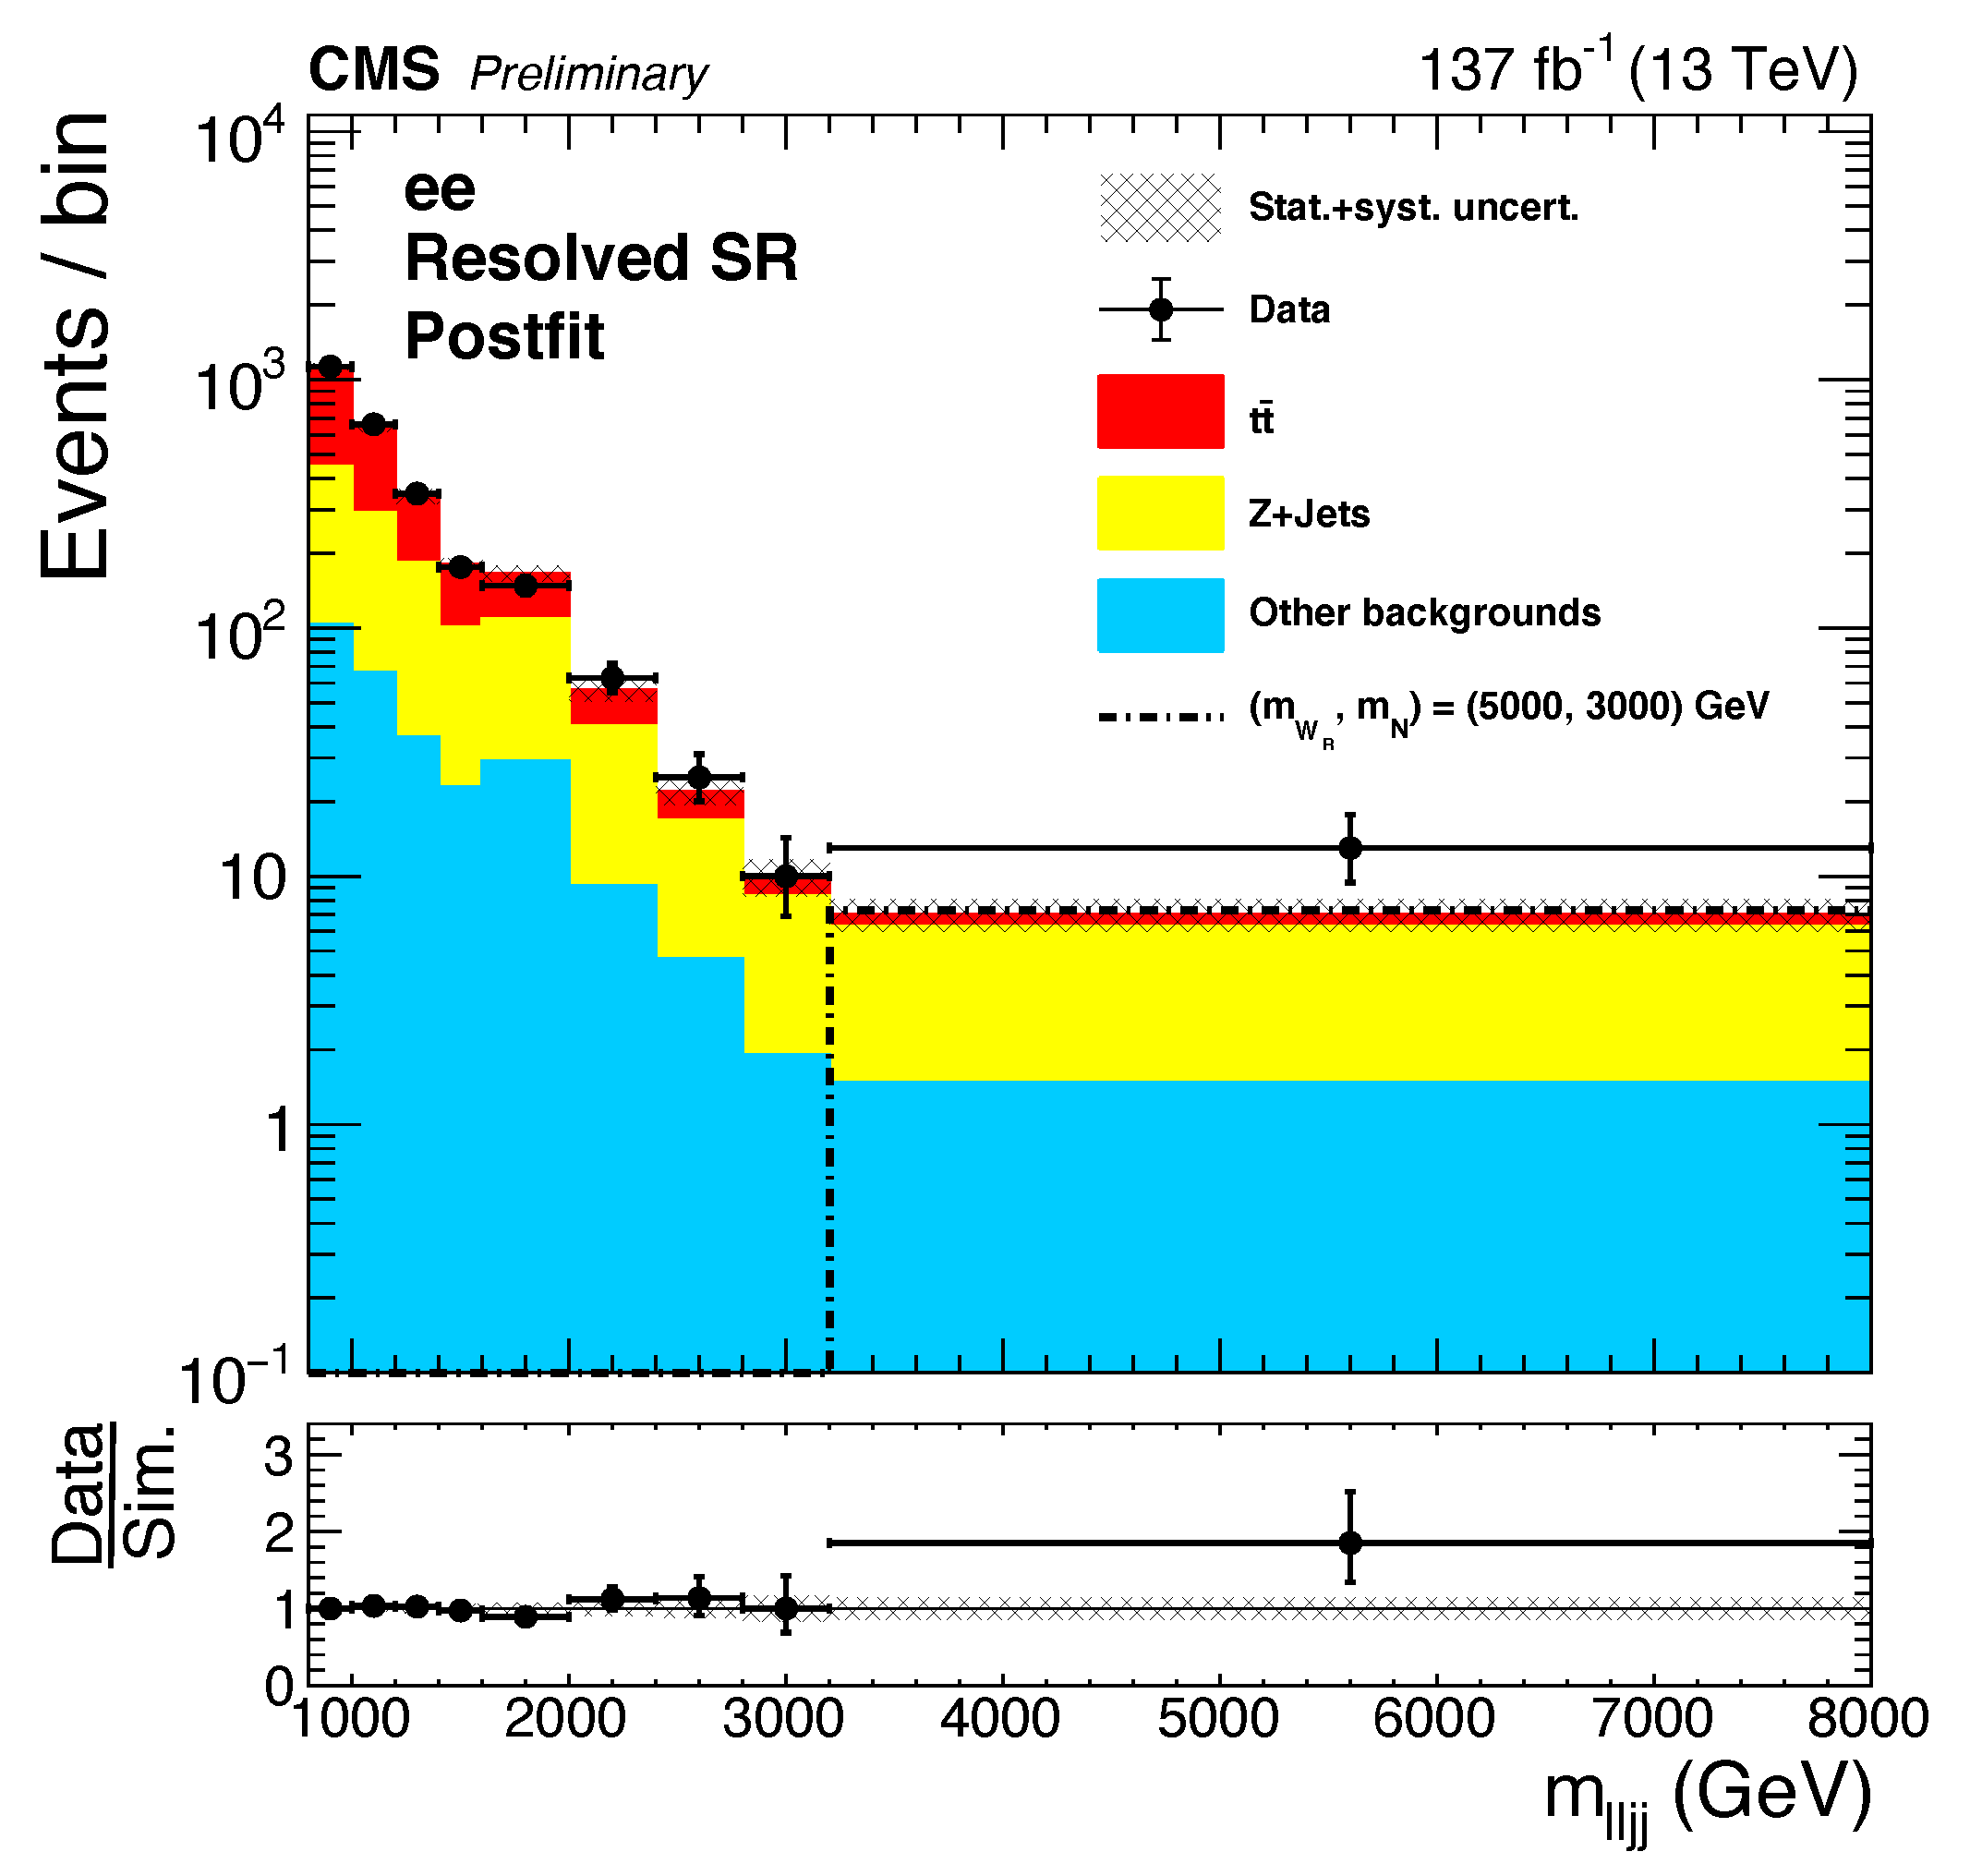
\includegraphics[width=\textwidth]{figures/Results/AllYears_PostFit_eeRes.pdf}
    \caption[
        %Short caption for the list of figures
       Multi-year resolved electron mass spectrum
    ]{
        % Full caption shown below the image
        The expected and measured mass spectrum is shown in the resolved electron channel. An excess can be seen in the last bin with 13 events observed and $\sim 8$ expected.
    }
    \label{fig:1Dlimit}
\end{figure}

While this excess could be indicative of some type of signal, it is important to additional study any possible reconstruction or detector effects as well as statistical error. With no observed excess in the muon channel, it is possible that the excess comes from an electron reconstruction or related detector issue (like the HEM failure). However, no significant suspects have been determined.



\label{ch:limit_setting}